\documentclass[crop,border=0pt]{standalone}

\usepackage{mathtools}
\usepackage{tikz}
\usetikzlibrary{positioning,scopes,arrows,shapes}

\begin{document}
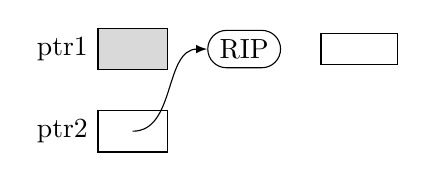
\begin{tikzpicture}[every node/.style={draw,minimum width=0.8cm}, node distance=0.5cm]
  \node [fill=gray!30] (ptr1) {\phantom{ptr1}};
  \node [right=of ptr1,rounded rectangle] (tomb) {RIP};
  \node [right=of tomb] (mem) {\phantom{mem}};
  \node [below=of ptr1] (ptr2) {\phantom{ptr2}};

  {[draw,-latex]
    \path (ptr2.center) edge [out=0,in=180] (tomb.west);
  }

  {[every node/.append style={draw=none}]
    \node [anchor=east] (ptr1 txt) at (ptr1.west) {ptr1};
    \node [anchor=east] (ptr2 txt) at (ptr2.west) {ptr2};
  }
\end{tikzpicture}
\end{document}
